\chapter{Grundlagen}

\section{Data Mining Frameworks}
Wie in Abschnitt \ref{sec:DataMining} bereits erwähnt, haben sich um das Data Mining drei bekannte Frameworks entwickelt. Diese werden im Nachfolgenden genauer betrachtet. Anschließend findet die Auswahl statt, welches Rahmenwerk Anwendung in dieser Arbeit findet.

\subsection{Knowledge Discovery in Databases (KDD) process model}
Die Bezeichung Knowledge Discovery in Databases wurde hauptsächlich von \citep{fayyad_data_1996} geprägt. Sie beschreiben in ihrer Arbeit ein Problem der 1990er Jahre. Wie auch heute noch, stieg damals die Masse der gespeicherten Daten exponentiell \todo{wirklich "exponentiell"?} an. Die Manuelle Auswertung dieser Datensätze erforderte mehr Arbeitskraft als vorhanden war. \citep[S.~38]{fayyad_data_1996} beschreiben es als "data overload". Deswegen versuchte man, die Prozesse zur Findung von Erkenntnissen zu automatisieren. Daraus hat sich ein Standardvorgehen entwickelt, dass das KDD-Prozessmodell darstellt.
\begin{figure}[H]
\frame{
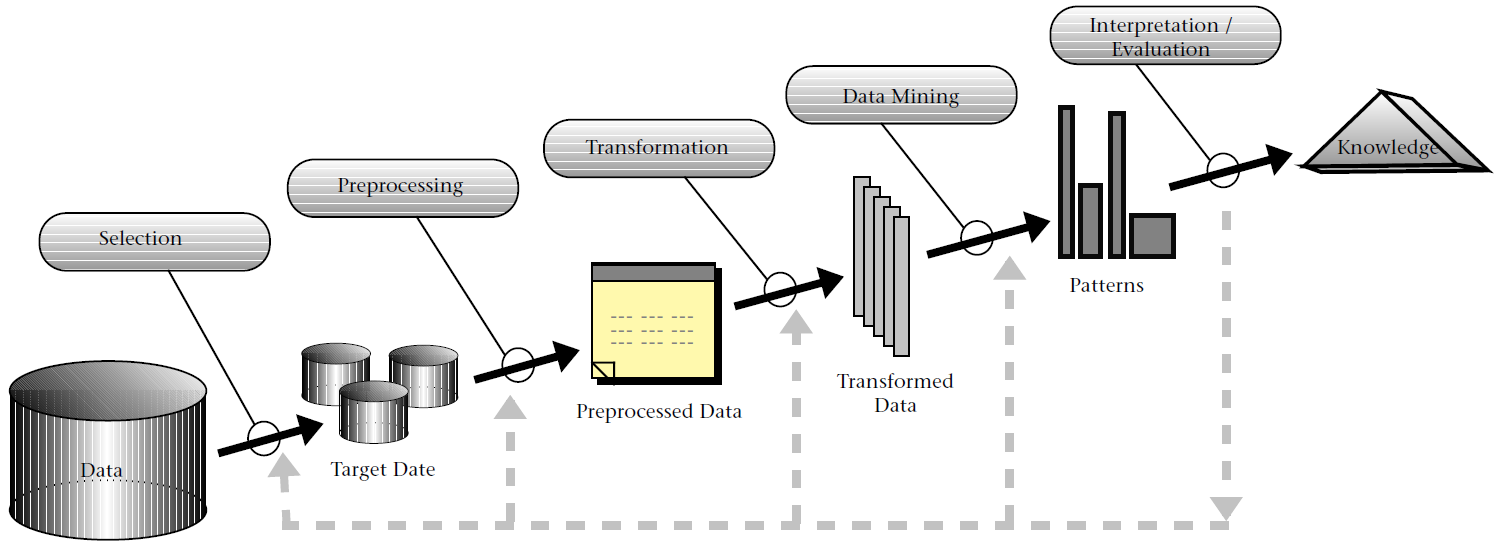
\includegraphics[width=\textwidth]{images/kddprocess}}
\caption{Ein Überblick über die Schritte des KDD Prozesses nach \citep[S.~41]{fayyad_data_1996}}
\label{fig:kddprocess}
\centering
\end{figure}


\subsubsection{Selection}
Bevor der erste eigentliche Schritt, die Selektion der Daten, erfolgen kann, ist es unabdingbar, ein "Verständnis für das Anwendungsgebiet zu entwickeln".\citep[S.~42; eigene Übersetzung]{fayyad_data_1996} Dies inkludiert auch, Ziele zu setzen und Fragen zu formulieren, die durch das spätere Data Mining (Schritt \ref{subsubsec:DataMining}) beantwortet werden sollen. \todo{wirklich "Ziele setzten"?} Ist das Verständnis hergestellt, kann ein "target data set"\citep[S.~42]{fayyad_data_1996} hergestellt werden. Dabei werden zuerst Daten aus unterschiedlichen - oft heterogenen - Quellen zusammengeführt und dann hinsichtlich des Ziels verdichtet.\citep[S.~70]{swamynathan_mastering_2017}

\subsubsection{Preprocessing}
Die verbleibende Teilmenge der ursprünglichen Daten muss nun noch gesäubert und für die nächsten Schritte vorbereitet werden. Dies geschieht, da unbereinigte Daten sowohl den Data Mining-Prozess verschlechtern können (unverlässliche oder falsche Ergebnisse), als auch die Zeit für das Mining deutlich verlängern können.\citep[S.~70]{swamynathan_mastering_2017}
Um die Qualität der Daten und des Mining zu verbessern, werden unter anderem folgende Aspekte betrachtet:\multicitep{fayyad_data_1996, S.~42; swamynathan_mastering_2017, S.~70}
\paragraph{Outliner treatment}\mbox{} \\
Ein Ausreißer (engl. outliner) kann beispielsweise ein "Extremer Wert in einer Variablen" oder ein "Extremer Wert des Residuums bei einer sinnvollen Regression"\citep[S.~25; Teil 5b]{hertle_datenanalyse_2016} sein. Ein Vorgehen für Ausreißer kann folgendermaßen aussehen (nach \citep[S.~25; Teil 5b]{hertle_datenanalyse_2016}):
\begin{enumerate}
\item Identifizieren der Ausreißer (evtl. durch eine erste Regression)
\item Interpretation im Sachzusammenhang (Messfehler oder wichtiger Teil der Population)
\item Entscheidung, ob man eine Regression der Daten mit oder ohne diese Ausreißer haben möchte
\item In der Darstellung der Ergebnisse auf die Ausreißer explizit eingehen und Vorgehen erläutern
\end{enumerate}

\paragraph{Noise removal}\mbox{} \\
Auch in einem Datensatz, der auf Ausreißer untersucht wurde, befinden sich immer noch unbekannte, unvollständige, falsche und fehlende Werte ("attribute noise"). Zusätzlich können Datenklassen falsch gekennzeichnet sein ("class noise"). Ist ein Datensatz von diesen Problemen betroffen, spricht man von "noisy data". Auf die Lösung dieses Problems wird an dieser Stelle nicht weiter eingegangen. 

\paragraph{Identifying duplicated values}\mbox{} \\
Wie oben angesprochen, wird der zu analysierende Datensatz aus mehreren Quellen zusammengeführt. Durch diesen Schritt können Datensätze doppelt (oder noch öfter) vorkommen. Das wird deutlich, wenn man folgendes Beispiel betrachtet: \newline
Über eine Kundenkarte werden Daten von Kunden eines Supermarkets je Filiale gespeichert. Bei einer überregionalen Kundenanalyse tauchen Kunden mehrfach auf, die in verschiedenen Filialen eingekauft haben. Hier ist anzumerken, dass doppelte Werte nicht zwangsläufig gelöscht werden müssen, sie sollten jedoch bei der Analyse bedacht werden.

\paragraph{Check for inconsistency}\mbox{} \\
Je größer ein Datensatz ist, umso wahrscheinlicher enthält der auch Inkonsistenzen \todo{quelle hierfür?}. Dies wird ebenfalls durch die Fusion von mehreren Quellen verstärkt (Beispiel: unterschiedliches Alter für einen Kundenstammsatz). Auch hier muss geprüft werden, wie mit diesen Werten umzugehen ist. Eventuell können Regeln festgelegt werden wie "immer der neuste Datenpunk ist der richtige".

\paragraph{Time series and changes}\mbox{} \\
Der letzte Punkt, der beim Preprocessing betrachtet werden muss, ist der Zusammenhang der Daten und dem Erfassungszeitpunkt. So können sich im Laufe der Zeit die Messmethodik (z.B. andere Sensoren), die Messgenauigkeit (z.B. bessere Sensoren) oder die Abstände der Messungen verändern. \todo{warum ist das schlecht: ungleich verteilte Datensätze/inkonsistente Genauigkeit}

\subsubsection{Transformation}
Der letzte Schritt vor dem eigentlichen Data Mining ist die Transformation. In diesem Prozessschritt geht es darum, "mit Dimensionsreduktions- oder -transformationsmethonden die effektive Anzahl an Variablen [...] zu reduzieren"\citep[S.~42; eigene Übersetzung]{fayyad_data_1996}. Dies geschieht beispielsweise durch das identifizieren und eliminieren invarianter Variablen. Ebenfalls wird versucht, solche Variablen zu finden, die mehrere Andere repräsentieren. Anschaulich dargestellt an einem Beispiel:\newline
\begin{table}[H]
\begin{tabular}{|rrrrrrr|}
  \hline
 & \textbf{Person} & \textbf{Studium} & \textbf{ErfahrungExtern} & \textbf{ErfahrungIntern} & \textbf{Alter} & \textbf{Gehalt} \\ 
\hhline{=======}
1 &   1 &   6 &   1 &   4 &  24 & 46450 \\ 
  2 &   2 &  18 &  30 &  15 &  55 & 85150 \\ 
  3 &   3 &  11 &   7 &   7 &  31 & 55900 \\ 
  4 &   4 &  11 &  15 &   8 &  36 & 63650 \\ 
  5 &   5 &  10 &   1 &  16 &  33 & 59050 \\ 
  6 &   6 &   6 &  25 &   6 &  38 & 68750 \\ 
  7 &   7 &  10 &  20 &  20 &  50 & 79000 \\ 
  8 &   8 &   7 &   0 &   1 &  23 & 43050 \\ 
   \hline
\end{tabular}
\caption{Einfacher Datensatz mit Berufserfahrung und Gehalt}
\label{tab:Beispiel_Berufserfahrung_R_output_simpleData}
\end{table}
Tabelle \ref{tab:Beispiel_Berufserfahrung_R_output_simpleData} zeigt einen einfachen Datensatz, in dem die Mitarbeiter einer Firma und die zugehörigen Gehälter festgehalten sind. "Studium" beschreibt die Anzahl der Halbjahre im Studium. Analog dazu "ErfahrungExtern" und "ErfahrungIntern" die Berufserfahrung in Halbjahren außerhalb und innerhalb der Firma. Zusätzlich ist das Alter der Personen gegeben.\newline
Führt man eine Regression (Listing \ref{list:Regression1}) für den Datensatz durch (mit Studium, ErfahrungExtern, ErfahrungIntern, Alter als unabhängige und Gehalt als abhängige Variablen), ergibt sich das Ergebnis in Tabelle \ref{tab:Regression1:output}.

\lstinputlisting[caption=Regression mit allen Faktoren,label=list:Regression1]{../R/Beispiel_Berufserfahrung/Regression1.R}

\begin{table}[H]
\begin{tabular}{|rrrrr|}
  \hline
 & \textbf{Estimate} & \textbf{Std. Error} & \textbf{t value} & \textbf{Pr($>$||)} \\ 
  \hhline{=====}
(Intercept) & 40000 & 1.415e-11 & 2.828e+15 & <2e-16 *** \\ 
  Studium & 300 & 5.167e-13 & 5.807e+14 & <2e-16 *** \\ 
  ErfahrungExtern & 850 & 4.821e-13 & 1.763e+15  & <2e-16 *** \\ 
  ErfahrungIntern & 950 & 6.308e-13 & 1.506e+15 & <2e-16 *** \\ 
  Alter & 2.010e-13 & 8.103e-13 & 2.480e-01 & 0.82 \\ 
\hline
\end{tabular}
\caption{Output der Regression mit allen Variablen}
\label{tab:Regression1:output}
\end{table}

Ohne weiter auf die genauen Beizeichnungen einzugehen, gibt die Sternnotation von R an, dass die unabhängigen Variablen Studium, ErfahrungIntern und ErfahrungExtern signifikant sind. Das Alter hingegen nicht. Die Regression hat ein adjustiertes Bestimmtheitsmaß ($R^2$; engl. adjusted R-squared) von 1. Das Bedeutet, dass das Gehalt vollständig durch die gegebenen Variablen erklärt werden kann (dies wird in der Realität jedoch nie erreicht).

\lstinputlisting[caption=Regression ohne Alter,label=list:Regression2]{../R/Beispiel_Berufserfahrung/Regression2.R}
\begin{table}[H]
\begin{tabular}{|rrrrr|}
  \hhline{=====}
 & \textbf{Estimate} & \textbf{Std. Error} & \textbf{t value} & \textbf{Pr($>$||)} \\
  \hline
(Intercept) & 40000 & 2.393e-12 & 1.671e+16 & <2e-16 *** \\ 
  Studium & 300 & 2.948e-13 & 1.018e+15 & <2e-16 *** \\ 
  ErfahrungExtern & 850 & 8.948e-14 & 9.500e+15 & <2e-16 *** \\ 
  ErfahrungIntern & 950 & 1.642e-13 & 5.787e+15.75 & <2e-16 *** \\ 
\hline
\end{tabular}
\caption{Output der Regression ohne Alters-Variable}
\label{tab:Regression2:output}
\end{table}
Führt man die Regression nun ohne das Alter durch (Listing \ref{list:Regression2} und Tabelle \ref{tab:Regression2:output}) bleibt $R^2$ gleich. Der Datensatz wurde also bereits um eine Variable reduziert, ohne das Ergebnis der Regression zu verschlechtern.\newline
Betrachtet man die Faktoren ErfahrungExtern und ErfahrungIntern, so fällt auf, dass sie einen ähnlichen Einfluss auf das Gehalte erzielen (850 und 950). 
\lstinputlisting[caption=Regression mit zusammengefassten Werten,label=list:Regression3]{../R/Beispiel_Berufserfahrung/Regression3.R}
Fasst man beide Variablen zusammen (Listing \ref{list:Regression3}), zeigt sich im Ergebnis (Tabelle \ref{tab:Regression3:output}), dass $R^2$ bei 0,9988 liegt. Die Güte der Regression hat sich also nur minimal verschlechtert.
\begin{table}[H]
\begin{tabular}{|rrrrr|}
  \hline
 & \textbf{Estimate} & \textbf{Std. Error} & \textbf{t value} & \textbf{Pr($>$||)} \\
  \hhline{=====}
(Intercept) & 40107.10 & 528.87 & 75.83 & 7.55e-09 *** \\
ErfahrungGesamt & 876.69 & 15.86 & 55.26 & 3.67e-08 ***\\ 
Studium & 327.17 & 64.27 & 5.09 & 0.0038 **\\ 
\hline
\end{tabular}
\caption{Output der Regression mit zusammengefassten Werten}
\label{tab:Regression3:output}
\end{table}
Zusammenfassend lässt sich für dieses Beispiel sagen, dass die Variablen im Datensatz um die Hälfte reduziert wurden, ohne die Aussagekraft deutlich zu verschlechtern. In einem realen Datensatz ist diese Arbeit zwar nicht so trivial und offensichtlich, jedoch gelten die gleichen Prinzipien.\newline
Nach \citep[S.~71; veränderte Version]{swamynathan_mastering_2017} gibt es zur Transformation folgende Möglichkeiten:
\begin{itemize}
\item Smoothing (binning, clustering, regression, etc.)
\item Aggregation (im Beispiel: das Zusammenfassen der Berufserfahrung)
\item Generalization (Ersetzen von primitiven Datenobjekten durch höherstufige Konzepte)
\item Normalization (min-max-scaling oder z-score)
\item Feature construction aus bereits bestehenden Attributen durch Techniken wie die Hauptkomponentenanalyse (engl. principal components analysis; PCA), Multidimensional scaling (MDS) oder Locally-linear embedding (LLE)
\item Compression (zum Beispiel wavelets, PCA, clustering etc.)
\item andere Datenreduzierungstechniken bei denen das Datenvolumen sinkt, ohne die Integrität der Originaldaten zu verletzten
\end{itemize}


\subsubsection{Data Mining}\label{subsubsec:DataMining}
Ist der Datensatz präpariert, so findet das eigentliche Data Mining statt. Dabei muss sich der Anwender für eine oder auch mehrere Methoden für das Mining entscheiden, um die anfänglichen Ziele zu erreichen und die Fragestellungen zu beantworten. Zur Auswahl stehen beispielsweise\multicitep{fayyad_data_1996, S.~42; swamynathan_mastering_2017, S.~71}:
\begin{itemize}
\item zusammenfassende und beschreibende Methoden: Mittelwert (arithmetisches Mittel), Median, Modus, Standardabweichung, Klassen-und Konzeptbeschreibungen, grafische Plots,
\item Vorhersagende Modelle (engl. predictive models): Klassifikationen und Regressionen und
\item Cluster-Analysen.
\end{itemize}
Eine genauere Beschreibung der Methoden (und der zugehörigen Algorithmen) im Kontext des Machine Learning befindet sich in Abschnitt \ref{sec:MachineLearning}. Je nach Beschaffenheit der zugrundeliegenden Daten und der gewählten Methode, muss ein passender Algorithmus gewählt und dieser korrekt parametrisiert werden. Zum Data Mining gehört auch, Hypothesen zu formulieren und das Ergebnis im Auge zu behalten: Ist der Endnutzer der Analyse an einem vorhersagenden Model interessiert (zum Beispiel für Wartungsarbeiten) oder an einem Jetzt-bezogenen (zum Beispiel für eine strategische Ausrichtung nach den aktuellen Kundensegmenten)?\newline
Anschließend erfolgt das (automatische) Mining der Daten. Je besser die vorhergehenden Schritte durchgeführt wurden, desto potenter ist das Ergebnis.\citep[S.~42]{fayyad_data_1996} Aus diesem Grund ist es auch jederzeit möglich, zu einem vorangegangen Prozessschritt zu springen, um neu erlangte Einsichten einfließen zu lassen (siehe zurückspringender grauer Pfeil in Abbildung \ref{fig:kddprocess}).

\subsubsection{Interpretation/Evaluation}
Zuletzt werden die gefundenen Muster und trainierten Modelle interpretiert. Ein Muster macht Aussagen über jeden Datenpunkt im betrachteten Raum. Ein Beispiel bei einem einfachen linearen Model: $$y = m \times x + t$$
Zu obigem Fall: $$Gehalt = Studium \times 327,17 + ErfahrungGesamt \times 876,69 + 40107,10$$ Ein Muster (engl. pattern) beschreibt dagegen nur eine kleine "lokale Struktur", die "nur über einen begrenzen Bereich" Aussagen macht.\citep[S.~71; eigene Übersetzung]{swamynathan_mastering_2017} Im Fall des linearen Model, wäre es eine bestimmte Gleichung, zum Beispiel $$y = 2 \times x + 5$$ oder $$ 6 \times 327,17 + 5 \times 876,69 + 40107,10 =  46453,57$$\citep{kraker_towards_2013}. "Fayyad et al. benutzt patterns und models synonym".\citep{kraker_towards_2013}\newline
Das Interpretieren der Ergebnisse beinhaltet ebenfalls das Zusammenfassen der Erkenntnisse und gegebenenfalls das Visualisieren.\citep[S.~71]{swamynathan_mastering_2017} Als Evaluieren wird das Eingliedern der Resultate in andere Systeme (zur Weiterverarbeitung oder Verbreitung), das Prüfen auf (und Lösen von) Konflikten mit anderen Untersuchungen und nicht zuletzt das Dokumentieren der Befunde bezeichnet.\citep[S.~42]{fayyad_data_1996} \newline
\todo{Befund nur medizinisch?; synonym)}
An dieser Stelle sei erneut angemerkt, dass das erste Ergebnis des KDD-Prozesses nicht das Endergebnis sein muss. Es kann durchaus viele Iterationen geben, die auch "loops between any two steps" beinhalten können.\citep[S.~42]{fayyad_data_1996}




\subsection{CRoss Industrial Standard Process for Data Mining (CRISP – DM)}
Bei CRoss Industrial Standard Process for Data Mining handelt es sich - wie bei KDD - um ein Referenzmodell für Data Mining. Das Modell wurde von einem 1996 gegründeten Konsortium aus "Daimler-Benz (now DaimlerChrysler), Integral Solutions Ltd. (ISL) [jetzt SPSS], NCR, and OHRA"\citep[S.~13]{shearer_crisp-dm_2000} erarbeitet. Die Version 1.0 wurde 2000 vorgestellt.\citep[S.~13]{shearer_crisp-dm_2000} In Umfragen (1999, 2002, 2004, 2007) wird das Modell als führend in Bereich von "data mining/predictive analytics projects"\citep[S.~72]{swamynathan_mastering_2017} bezeichnet. Das Modell ist "nicht-properitär, dokumnetiert und frei verfügbar"\citep[S.~13; eigene Übersetzung]{shearer_crisp-dm_2000}. Es ist ebenfalls in vielen Bereichen nutzbar, da es weder Industriesektor-, Werkzeugs- noch Anwendungsspezifisch ist. Grundsätzlich bekräftigt das Modell best practices und soll zu besseren und schnelleren Ergebnissen führen.\citep[S.~13; eigene Übersetzung]{shearer_crisp-dm_2000} \todo{evtl. bessere Bezeichnung}\newline 


\begin{figure}[H]
\frame{
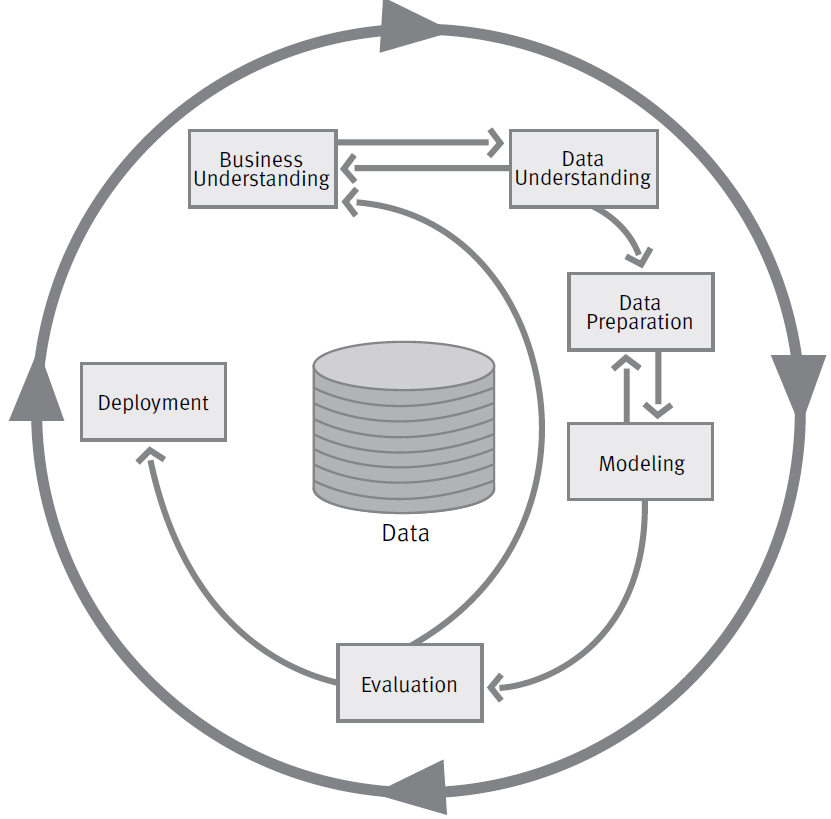
\includegraphics[width=\textwidth]{images/CRISP_DM}}
\caption{Phasen des CRISP-DM Referenzmodells nach \citep[S.~10]{chapman_crisp-dm_2000}}
\label{fig:CRISP_DM}
\centering
\end{figure}

Wie in Abbildung \ref{fig:CRISP_DM} zu sehen ist, umfasst das Referenzmodell sechs Phasen. Genau wie beim KDD-Prozessmodell handelt es sich nicht um ein lineares Modell, sondern um eines, das Rückschritte und Iterationen erlaubt. Im Nachfolgenden wird zuerst immer ein Prozessschritt kurz vorgestellt und darunter detaillierter betrachtet. Als Referenz dient unter anderem Abbildung \ref{fig:CRISP_DM_detailed}, die zusätzlich den Output der einzelnen Schritte zeigt.

\begin{figure}[H]
\frame{
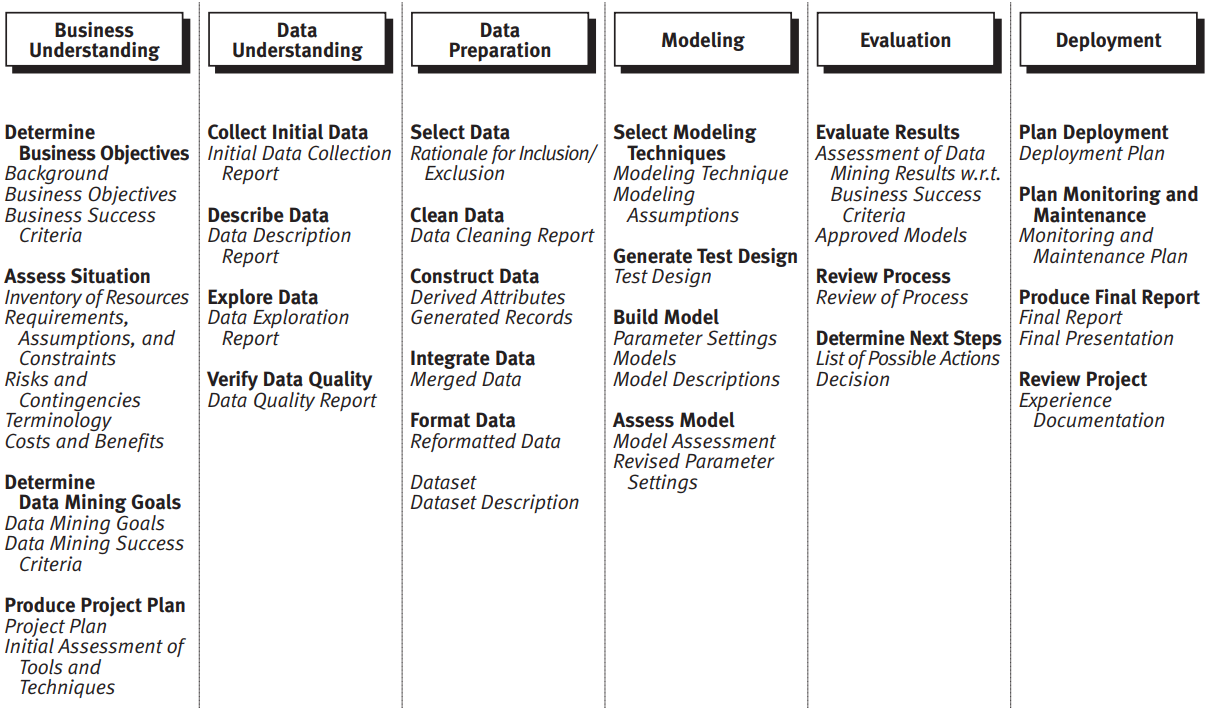
\includegraphics[width=\textwidth]{images/crisp_dm_detailed}}
\caption{Generische Aufgaben (bold) und Output (italic) des CRISP-DM Referenzmodells \citep[S.~12]{chapman_crisp-dm_2000}}
\label{fig:CRISP_DM_detailed}
\centering
\end{figure}

\subsubsection{Business Understanding}
Die erste und vielleicht wichtigste Phase\citep[S.~14]{shearer_crisp-dm_2000} des CRISP-DM Prozesses ist das "Business Understanding", oder auch "Research Understanding"\citep[Punkt 1.4.1.1]{larose_discovering_2014}. Die Aufgabe dieser Phase ist, die "Ziele und Erwartungen"\citep[S.~73]{swamynathan_mastering_2017} des Projektes zu verstehen, dieses "Wissen in eine Machine Learning Problem Definition zu übersetzen" und schließlich einen "Vorläufigen Plan"\citep[S.~14]{shearer_crisp-dm_2000} aufzustellen: 
\paragraph{Determine the Business Objectives}\mbox{} \\
Dieser Teilschritt soll hauptsächlich die Frage beantworten, warum die Analyse durchgeführt wird. Dies hat direkten Einfluss auf die Zeile des Projekts und soll verhindern, dass "viel Aufwand für das Finden von richtigen Antworten auf falsche Fragen"\citep[S.~14]{chapman_crisp-dm_2000} verschwendet wird.
\paragraph{Assess the Situation}\mbox{} \\
Um das Ziel der Analyse so genau wie möglich zu treffen, muss genau nachgeforscht werden, welche Ressourcen verfügbar sind, welchen Zwängen und Grenzen die Analyse unterlegen ist und unter welchen Annahmen sie stattfindet.\citep[S.~14]{chapman_crisp-dm_2000} Vereinfacht lässt sich sagen, dass hier die Fragen aus dem vorhergehenden Schritt detaillierter betrachtet werden.
\paragraph{Determine the Data Mining Goals}\mbox{} \\
Die gefundenen Ziele sind meist in Geschäftssprache formuliert. Für die Analyse müssen die Ziele jedoch im Terminus technicus des Data Mining formuliert sein. Ein Beispiel dazu ist die Übersetzung von "Increase catalog sales to existing customers." in "Predict how many widgets a customer will buy, given their purchases over the
past three years, demographic information (age, salary, city, etc.), and the price of the item."\citep[S.~16]{chapman_crisp-dm_2000}
\paragraph{Produce a Project Plan}\mbox{} \\
Der Projektplan (engl. Project Plan) liefert einen konkreten Plan, wie die gesetzten Ziele zu erreichen sind. Nach \citep[S.~15]{shearer_crisp-dm_2000} beinhaltet er:
\begin{itemize}
\item Die Schritte, die nacheinander durchzuführen sind.
\item Eine Timeline \todo{richtiges Wort?} für die Durchführung.
\item Eine Auflistung potentieller Risiken im Projektverlauf.
\item Eine Aufstellung der zu nutzenden Werkzeuge und Techniken \citep[S.~16]{chapman_crisp-dm_2000}
\end{itemize}


\subsubsection{Data Understanding}
In der vorhergegangenen Phase wurde festgelegt, welche Daten zum erreichen der Ziele benötigt werden. Nun werden diese Daten gesammelt und untersucht. Im Fokus der Untersuchung liegt dabei\citep[S.~73]{swamynathan_mastering_2017}
\begin{itemize}
\item Datenlücken finden,
\item die Relevanz der erfassten Daten (hinsichtlich der Ziele) zu klären,
\item die allgemeine Datenqualität festzustellen und
\item "erste Einblicke in Daten" zu erhalten, um "geeignete Hypothesen"\citep[S.~73; eigene Übersetzung]{swamynathan_mastering_2017} zu formulieren.
\end{itemize}
Im Zuge dessen können auch bereits "subsets" isoliert werden, die "actionable patters"\citep[Punkt 1.4.1.2.d]{larose_discovering_2014} (etwa: verfolgbare Muster) enthalten könnten. Mit jedem Fortschritt in dieser Phase ist es eventuell nötig, das Ergebnis der Business Understanding-Phase zu adjustieren. Durch dieses Vorgehen, entsteht ein iterativer Prozess.\citep[S.~73]{swamynathan_mastering_2017} \citep[Punkt 1.4.1.2.b]{larose_discovering_2014} empfiehlt den Einsatz von explorativer Datenanalyse (siehe Abschnitt \ref{sec:DataMining}). 


\paragraph{Collect the Initial Data}\mbox{} \\
Die Hauptaufgabe dieses ersten Schrittes ist, die benötigten Daten zu beziehen. Dabei kann auch entweder der direkte Zugriff auf die Daten gemeint sein oder nur das Erhalten der Zugangsinformationen. Eventuell werden die Datensätze gleich in Systeme oder Werkzeuge geladen, die zur späteren Weiterverarbeitung genutzt werden. Die Integration inhomogener Daten (unterschiedliche Strukturen/Formate etc.) kann bereits hier erfolgen oder in der Data Preperation (siehe Punkt \ref{subsubsec:DataPreperation}). \citep[S.~18]{chapman_crisp-dm_2000}

Sollten in diesem Schritt Probleme auftauchen, sollten sie - wenn möglich mit Lösung - gut dokumentiert werden, um den Projektverlauf reproduzierbar zu gestalten. Ein Beispiel können lange Antwortzeiten einiger Datenquellen sein.\citep[S.~15]{shearer_crisp-dm_2000}

\paragraph{Describe the Data}\mbox{} \\
Im Schritt "Describe the Data" werden die beschafften Daten dann oberflächlich beschrieben.\citep[S.~18]{chapman_crisp-dm_2000} Dabei wird unter anderem auf 
\begin{itemize}
\item das Format der Daten,
\item die Größe des Datensatzes,
\item die Anzahl der Beobachtungen und Einträge in den Daten und 
\item die Beschaffenheit der Einträge
\end{itemize}
geachtet. Dabei soll einerseits die Frage geklärt werden, ob die vorhandenen Daten alle relevanten Daten für die Ziele des Data Mining enthalten. Andererseits wird das Verständnis der Daten geschärft.\citep[S.~15]{shearer_crisp-dm_2000}

Anhand des nachfolgenden Beispiels (Datensatz von \citep[Case Lasagne Test.xlsx]{hertle_datenanalyse_2016}) werden die Schritte "Collect the Initial Data" und "Describe the Data" kurz visualisiert. Zuerst werden die Daten eingelesen (Listing \ref{list:LasagneHead}) und anschließend oberflächlich betrachtet.
\lstinputlisting[caption=Einlesen aller Daten und Betrachten des "Kopfes" ,label=list:LasagneHead]{../R/Beispiel_Head_Lasagne/head_lasagne.R}
Aus Tabelle \ref{tab:LasagneHead:output} kann abgelesen werden, dass es sich um einen Datensatz mit 12 Variablen handelt. 
\begin{table}[H]
\centering
\begin{tabular}{|p{1cm}p{0.7cm}p{1.2cm}p{1.9cm}p{1.6cm}p{1.7cm}p{3.5cm}p{1.8cm}|}
  \hline
\textbf{Person} & \textbf{Alter} & \textbf{Gewicht} & \textbf{Einkommen} & \textbf{Angestellt} & \textbf{Wert.Auto} & \textbf{Umsatz.Kreditkarte} & \textbf{Geschlecht} \\ 
  \hhline{========}
1 &  48 &  65 & 91700 & nein & 2190 & 3510 & m\\ 
2 &  33 &  75 & 40740 & nein & 2110 & 740& w\\ 
3 &  51 &  70 & 45080 & ja & 5140 & 910 & m\\ 
4 &  56 &  91 & 26600 & nein & 700 & 1620 & w\\ 
5 &  28 &  81 & 113960 & ja & 26620 & 600 & m\\ 
6 &  51 &  65 & 102200 & ja & 24520 & 950 & w\\ 
\hline
\end{tabular}
\begin{tabular}{|p{2.2cm}p{2.1cm}p{5.8cm}p{3cm}|}
  \hline
\textbf{alleinstehend} & \textbf{Wohnung} & \textbf{Supermarkt.besuche.pro.Monat} & \textbf{Lasagne.probiert}\\ 
  \hhline{====}
nein & Haus &   7 & nein\\ 
nein & Wohnung &   4 & ja\\ 
nein & Wohnung &   1 & nein\\ 
nein & Haus &   3 & nein\\ 
nein & Appartement &   3 & ja\\ 
nein & Wohnung &   2 & nein\\ 
   \hline
\end{tabular}
\caption{Aufruf des head()-Befehls zum Betrachten der Daten}
\label{tab:LasagneHead:output}
\end{table}
Ebenfalls entnommen werden kann, dass es sich um demographische Angaben über Personen handelt. Zusätzlich wurde zu jeder Person erfasst ob sie Lasagne probiert hat. In Abbildung \ref{fig:Lasagne_RStudio} wird der Datensatz schließlich in RStudio betrachtet.
\begin{figure}[H]
\frame{
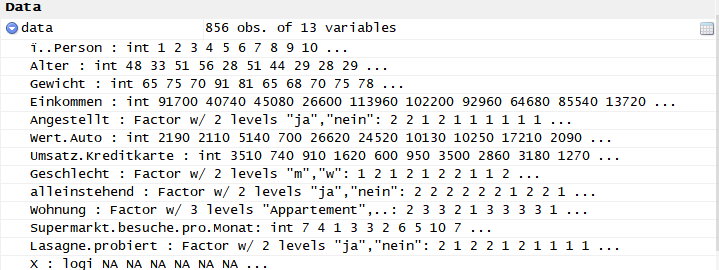
\includegraphics[width=\textwidth]{images/Lasagne_data}}
\caption{Betrachten der Datentypen des Datensatzes in RStudio}
\label{fig:Lasagne_RStudio}
\centering
\end{figure}
Zu sehen ist hier, dass es sich um einen Datensatz mit 13 Variablen und 856 Beobachtungen handelt (hier scheint ein falscher Zeichensatz vorzuliegen oder Ähnliches, da eine zusätzliche leere Spalte "X" angezeigt wird \todo{was hier tun?}). Zusätzlich können die vorgeschlagenen Datentypen von R betrachtet werden. Bei den meisten Spalten handelt es sich um Ganzzahlen (int) oder Factoren (manchmal auch als Enums bezeichnet).

\paragraph{Explore the Data}\mbox{} \\
Ist die grobe Sichtung der Daten abgeschlossen, wird näher an der Fragestellung des Data Mining gearbeitet. Dazu werden "Abfrage-, Visualisierungs- und Reporting[-Techniken]"\citep[S.~16; eigene Übersetzung]{shearer_crisp-dm_2000} eingesetzt. Um der Antwort auf die ursprüngliche Fragestellung näher zu kommen oder die Fragestellung zu verfeinern, werden beispielsweise folgende Eigenschaften betrachtet\citep[S.~18; eigene Übersetzung]{chapman_crisp-dm_2000}:
\begin{itemize}
\item Die Verteilung der Schlüsselattribute (zum Beispiel der Zielvariablen bei einer Vorhersage).
\item Die Beziehungen zwischen Wertepaaren oder kleinen Attributgruppen.
\item Die Ergebnisse einfacher Aggregationen.
\item Die Beschaffenheit von aussagekräftigen Teilgruppen von Werten.
\item Die Ergebnisse einfacher statistischer Analysen.
\end{itemize}

\paragraph{Verify Data Quality}\mbox{} \\
Der letzte Schritt der zweiten Phase evaluiert die Qualität der Daten. \citep[S.19]{chapman_crisp-dm_2000} nutzen die Zielfragen: 
\begin{itemize}
\item "Is the data complete (does it cover all the cases required)?"
\item "Is it correct, or does it contain errors and, if there are errors, how common are they?"
\item "Are there missing values in the data?"
\item "If so, how are they represented, where do they occur, and how common
are they?"
\end{itemize}
\citep[S.~16]{shearer_crisp-dm_2000} empfiehlt zusätzlich noch, zu prüfen, ob die Werte plausibel sind, wie die Schreibweisen sind, ob Attribute mit unterschiedlichen Werten aber gleicher Bedeutung vorhanden sind und schließlich ob es einen "conflict with common sense" ,wie "teenagers with high income"\citep[S.~16]{shearer_crisp-dm_2000} gibt. 
\subsubsection{Data Preparation}\label{subsubsec:DataPreperation}
In der aufwendigsten Phase des ganzen Prozesses (siehe Abbildung \ref{fig:CRISP_DM_percent}) wird das "final data set"\multicitep{larose_discovering_2014, Punkt 1.4.1.3.a; shearer_crisp-dm_2000, S.~16} erzeugt. Dies geschieht durch\citep[S.~73]{swamynathan_mastering_2017}
\begin{itemize}
\item generelle Transformationen,
\item Füllen der Datenlücken, die in vorhergehenden Schritten aufgedeckt wurden,
\item Befassen mit fehlenden Werten,
\item Herausarbeiten, welche Features des Datensatzes die größte Relevanz haben und welche neuen Features sinnvoll wären.
\end{itemize}
Wie bereits erwähnt, handelt es sich nicht nur um die Phase, die den meisten Aufwand erfordert, sondern auch um die, von der die Genauigkeit des Endresultates zu großen Stücken abhängt.\citep[S.~73]{swamynathan_mastering_2017}

\begin{figure}[H]
\frame{
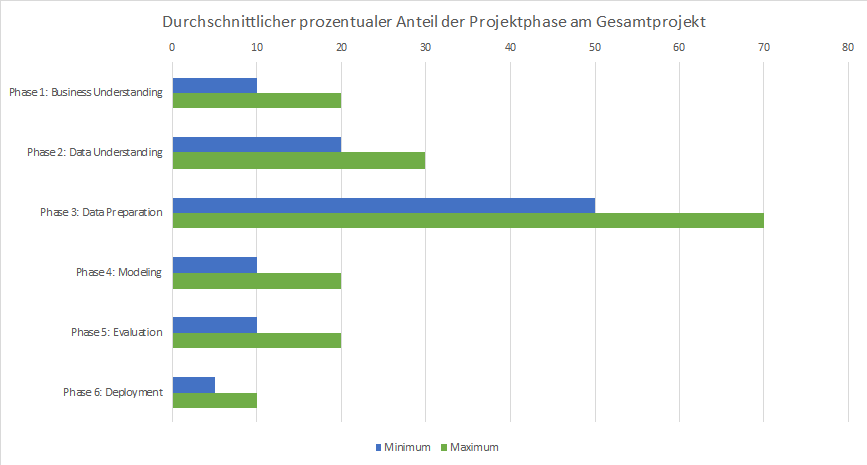
\includegraphics[width=\textwidth]{images/ProjektphasenInProzent_DRISP_DM}}
\caption{Durchschnittlicher prozentualer Anteil der CRISP-DM-Projektphase am Gesamtprojekt nach \citep[S.~15; eigene Darstellung]{shearer_crisp-dm_2000}}
\label{fig:CRISP_DM_percent}
\centering
\end{figure}

\paragraph{Select Data}\mbox{} \\
Genauer wird dabei im ersten Schritt ausgewählt, welche Daten Teil der Analyse bleiben und welche exkludiert werden. Kriterien sind dabei, die Relevanz hinsichtlich der Ziele, die Qualität der Daten und technische Grenzen\citep[S.~16]{shearer_crisp-dm_2000} (wie "data volume or data types"\citep[S.~21]{chapman_crisp-dm_2000}). Zusätzlich kann überlegt werden, ob einige Attribute wichtiger sind als andere. So kann beispielsweise bei einer landesweiten Kundenanalyse die Postleitzahl der Kunden ausreichen und Straße und Hausnummer vernachlässigt werden.\citep[S.~16]{shearer_crisp-dm_2000} \citep[S.21]{chapman_crisp-dm_2000} merken an, dass diese Phase sowohl "attributes (columns)", als auch "records (rows)" umfasst. Wie bereits in den vorhergehenden Schritten muss auch hier erklärt werden, warum Entscheidungen getroffen wurden und eine Dokumentation angefertigt werden.\citep[S.~16]{shearer_crisp-dm_2000}

\paragraph{Clean Data}\mbox{} \\
Im Schritt "Verify Data Quality" wurde herausgearbeitet, wie die Qualität der Daten ist \todo{bessere Formulierung} und wie mängelbehaftet sie sind. Jetzt werden Maßnahmen dagegen ergriffen. Neben trivialen Vorgehen wie "Auswahl von reinen Untermengen" oder "Einfügen von passenden Standardwerten" können "anspruchsvollere Techniken wie das Schätzen von fehlenden Werten"\citep[S.21; eigene Übersetzung]{chapman_crisp-dm_2000} zum Zuge kommen.

\paragraph{Construct Data}\mbox{} \\
Die gereinigten Daten sind noch nicht fertig für die Modeling-Phase. Manchmal ist es notwendig, einem Datensatz neue Zeilen hinzuzufügen. Betrachtet man wieder eine Kundenanalyse, so ist es vielleicht nötig, für einen Kunden, der in einem Quartal keinen Einkauf getätigt hat, einen leeren Einkauf (null Euro) anzulegen, falls der eingesetzte Algorithmus dies erfordert.\citep[S.~22]{chapman_crisp-dm_2000} Er kann auch verlangen, dass abgeleitete  statt der Ursprungswerte benötigt werden. Dabei gibt es nach \citep[S.~16]{shearer_crisp-dm_2000} zwei Fälle:
\begin{enumerate}
\item Wenn zu einem Kunden ein Bewegungsprofil vorhanden ist (in welchem Geschäft er einkaufen war), so ist möglicherweise sinnvoll, nicht das gesamte Profil zu betrachten, sondern lediglich die Fläche zu betrachten, in der er sich bewegt hat.
\item Ebenfalls zielführend kann eine "single-attribute transformation" sein. Dabei wird beispielsweise das genaue alter der Kunden in Altersspannen umgewandelt oder sprechende Werte wie "("definitely yes," "yes," "don't know," "no")" in numerische Werte übersetzt.
\end{enumerate}
\citep[S.~16; eigene Übersetzung]{shearer_crisp-dm_2000} merkt aber auch an, dass es nicht immer sinnvoll ist dies zu tun, auf jeden Fall "nicht nur um die Anzahl der Inputattribute zu reduzieren."

\paragraph{Integrate Data}\mbox{} \\
Der vorletzte Schritt der Data Pereperation ist das Zusammenführen von mehren Quellen oder Tabellen mit dem gleichen Thema. Dadurch können "neue Beobachtungen oder Werte"\citep[S.~22]{chapman_crisp-dm_2000} gewonnen werden. In Tabelle \ref{tab:integrateData} werden die zwei Hauptaufgaben\citep[S.~17]{shearer_crisp-dm_2000} genauer erläutert.
\begin{table}[H]
\begin{tabular}{|p{2cm}|p{3.5cm}|p{10cm}|}
\hline
\textbf{Aufgabe} & \textbf{Erläuterung} & \textbf{Beispiel}\\
\hhline{===}
Join & Mehrere Tabellen zum gleichen Thema werden zusammengeführt. & Die drei Ausgangstabellen
\begin{itemize}
\item "information about each store’s general characteristics (e.g., floor space, type of mall)"
\item "summarized sales data (e.g., profit, percent change in sales from previous year)"
\item "information about the demographics of the surrounding area"
\end{itemize}
werden in 
\begin{itemize}
\item "a new table with one record for each store, combining fields from the source tables"\citep[S.~16]{shearer_crisp-dm_2000}
\end{itemize}
zusammengeführt. \\ \hline
Aggregation &  Errechnen neuer Werte aus Informationen verschiedener Tabellen. & Das Überführen von einer
\begin{itemize}
\item "table of customer purchases, where there is one record for each purchase"
\end{itemize}
in eine 
\begin{itemize}
\item "new table where there is one record for each customer"
\end{itemize}
mit den Feldern 
\begin{itemize}
\item "number of purchases, the average purchase amount, the percent of orders charged to credit cards, the
percent of items under promotion, etc".\citep[S.~17]{shearer_crisp-dm_2000}
\end{itemize}
\\
   \hline
\end{tabular}
\caption{Die zwei Hauptaufgaben des Schrittes Integrate Data}
\label{tab:integrateData}
\end{table}

\paragraph{Format Data}\mbox{} \\
Die Datenformatierung umfasst "hauptsächlich syntaktische Abänderungen" und "verändert nicht die Bedeutung"\citep[S.~22; eigene Übersetzung]{chapman_crisp-dm_2000} der Daten. Das kann kann zum Beispiel das "Entfernen von unerlaubten Zeichen in Zeichenketten"\citep[S.~17; eigene Übersetzung]{shearer_crisp-dm_2000} sein.\newline
Mit diesem Schritt ist die Data Preperation abgeschlossen und es kann mit dem Modeling begonnen werden.

\subsubsection{Modeling}
Die Phase des Modeling umfasst die Auswahl einer oder mehrerer Data Mining-Algorithmen, die Optimierung ihrer Parameter und Settings und der Evaluierung des erzeugten Models.\multicitep{swamynathan_mastering_2017, S.~73; larose_discovering_2014, Punkt 1.4.1.4} Eventuell muss der Datensatz noch angepasst werden, sodass die Data Preperation-Phase noch einmal durchlaufen werden muss.\citep[Punkt 1.4.1.4]{larose_discovering_2014}

\paragraph{Select the Modeling Technique}\mbox{} \\
Wie der Name des ersten Schrittes bereits andeutet, wird eine Modellierungstechnik ausgewählt. Werden mehrere Techniken ausgewählt, so wird diese Phase mehrfach (parallel) durchlaufen. Wichtig ist hier, dass getroffene Annahmen (wie "alle Attribute sind stetig Gleichverteilt" oder "fehlende Werte sind nicht zugelassen"\citep[S.~24]{chapman_crisp-dm_2000}) dokumentiert werden.\citep[S.~17]{shearer_crisp-dm_2000}

\paragraph{Generate Test Design}\mbox{} \\
Vor der eigentlichen Modellierung wird festgelegt, wie die "Qualität und Validität"\citep[S.~24]{chapman_crisp-dm_2000} festgestellt werden soll. Für "supervised data mining" werden dabei meist "error rates"\citep[S.~24]{chapman_crisp-dm_2000} herangezogen. Dazu wird das Modell mit einem Datensatz (train set) trainiert und mit einem anderen (test set) getestet.\citep{shearer_crisp-dm_2000}

\paragraph{Build the Model}\mbox{} \\
Der kürzeste Schritt dieser Phase ist "Build the Model". Hier wird das Model mit Hilfe eines - möglichweise vorher bereits gewählten - Werkzeuges erzeugt.\multicitep{chapman_crisp-dm_2000, S.~24; shearer_crisp-dm_2000, S.~17} Wurden zwei Schritte zuvor mehrere Modellierungstechniken ausgewählt, so liegen an dieser Stelle mehrere Models vor.

\paragraph{Assess the Model}\mbox{} \\
Ist das Modellieren abgeschlossen, werden die Ergebnisse auf Basis 
\begin{itemize}
\item des Verständnisses aus der ersten Phase (Business Understanding),
\item der Data Mining-Ziele und
\item des Test Designs aus dieser Phase
\end{itemize}
interpretiert. Der Analyst hat die Aufgabe, den Grad des Erfolgs des Data Mining zu bestimmen. Dazu kann er Experten heranziehen, um das Ergebnis beispielsweise auf Geschäftsebene zu diskutieren. Zusätzlich wird eine Rangliste aller Modelle aufgestellt, die den Erfolg hinsichtlich der "Business Ziele" (aus Phase "Business Understanding", Schritt "Determine the Business Objectives") abbildet.\multicitep{chapman_crisp-dm_2000, S.~25; shearer_crisp-dm_2000, S.~17} \newline
In diesem Schritt werden die Modelle ein erstes Mal interpretiert. \todo{bessere Wortwahl als "interpretiert"} Eine genauere Evaluation und zusätzliche Ergebnisse, Erkenntnisse und Dokumente aus den vorhergehenden Schritten werden in der nachfolgenden Evaluation-Phase bewertet.\citep[S.25]{chapman_crisp-dm_2000}


\subsubsection{Evaluation}
Die Tatsache, dass es sich beim CRISP-DM-Referenzmodell um einen Prozess handelt und nicht um strikt getrennte Einzelschritte, wird besonders in der Evaluations-Phase deutlich. Erstens wird das Ranking aus dem vorherigen Schritt in in einem "Benchmarking" über die "Models mit einer hohen Genauigkeit"\citep[S.~73; eigene Übersetzung]{swamynathan_mastering_2017} verfeinert. Zweitens werden die Models erneut mit frischen Daten (nicht aus Schritt "Generate Test Design") verifiziert und gegen die Business-Anforderungen aus Phase 1 geprüft.\citep[S.~73]{swamynathan_mastering_2017} Ziel dieser Phase ist vor allem, dem Projektleiter genug Wissen an die Hand zu geben, um zu Entscheiden, wie mit den Ergebnissen des ganzen Prozesse weiter verfahren wird. 

\paragraph{Evaluate Results}\mbox{} \\
Während sich bisher hauptsächlich um die "Genauigkeit und Allgemeingültigkeit" der Modelle gekümmert wurde, wird jetzt auch betrachtet, ob es "irgendwelche Businessgründe gibt", durch die das Model "mangelhaft"\citep[S.~18; eigene Übersetzung]{shearer_crisp-dm_2000} wird. Falls "time und budget"\citep[S.~26]{chapman_crisp-dm_2000} es erlauben, können die Ergebnisse bereits in echte Systeme in Testumgebungen implementiert werden. Wie bereits angemerkt, werden in dieser Phase auch andere "findings" evaluiert, die beispielsweise auf zukünftige Herausforderungen hinweisen.\citep[S.~18]{shearer_crisp-dm_2000} Ist dies geschehen, "fasst der Data Analyst die Bewertungen der Ergebnisse hinsichtlich der geschäftlichen Erfolgskriterien zusammen" und gibt seine Wertung ab, "ob das Projekt bereits die initialen geschäftlichen Ziele erreicht"\citep[S.~18; eigene Übersetzung]{shearer_crisp-dm_2000}.

\paragraph{Review Process}\mbox{} \\
Im Review wird abgesichert, dass kein Faktor unbeachtet geblieben ist und keine Aufgabe vergessen wurde. Ebenfalls wird die Qualität gesichert (zum Beispiel Bugs in Softwarekomponenten gesucht) und rechtliche Überlegungen angestellt ("Dürfen wir diese Kundendaten produktiv für diese Analyse benutzen?").\multicitep{shearer_crisp-dm_2000, S.~18; chapman_crisp-dm_2000, S.~27}

\paragraph{Determine Next Steps}\mbox{} \\
Schließlich werden alle Bewertungen bis hierher genutzt, um zu entscheiden, ob eine weitere Prozessiteration durchlaufen wird, oder, ob in die Deployment-Phase übergegangen wird. Laut \citep[S.~18]{shearer_crisp-dm_2000} trifft diese Entscheidung der Projektleiter. \citep[S.~17]{chapman_crisp-dm_2000} sind der Meinung, dass das ganze Projektteam entscheiden sollte.

\subsubsection{Deployment}
Ist die Entscheidung für das Deployment gefallen, wird die letzte Phase initiiert. Zu Beginn des CRISP-DM-Prozesses wurden Ziele festgelegt, die begründen, weshalb das Data Mining durchgeführt werden soll. 
Eine einfache Implementierung wäre das Erstellen eines Reports, eine Komplexere dagegen, den Data Mining Prozess in eine andere Abteilung zu portieren\citep[Punkte 1.4.1.6.b und c]{larose_discovering_2014} oder "Echtzeit-Personalisierung von Webseiten"\citep[S.~18; eigene Übersetzung]{shearer_crisp-dm_2000} durchzuführen.\newline
Die Implementierung des Models in die produktiven Systeme befriedigt diese Ziele nicht alleine. Auch das Training jener Personen, die das Wissen im Geschäftsprozess anwenden, muss durchgeführt werden. Dies beinhaltet sowohl die Fähigkeit, die Ergebnisse zu interpretieren, als auch zu verstehen, wie sie die Entscheidungsfindung unterstützen können.\citep[S.~73]{swamynathan_mastering_2017} \newline

Da die weiteren Aufgaben oft nicht vom Data Analyst durchgeführt werden \citep[Punkt 1.4.1.6.d]{larose_discovering_2014}, muss der Anwender die Pflege eines Machine Learning-Models verstehen und übernehmen (z.B. in welchen Intervallen das Model trainiert wird).\citep[S.~74]{swamynathan_mastering_2017}

\paragraph{Plan Deployment}\mbox{} \\
Der Erste Schritt  der Deploymentphase ist die Auswahl und Dokumentation einer geeigneten Strategie für den Einsatz oder das Rollout in die Geschäftsumgebung.\multicitep{shearer_crisp-dm_2000, S.~18; chapman_crisp-dm_2000, S.~28} \todo{Formulierung}. 

\paragraph{Plan Monitoring and Maintenance}\mbox{} \\
Zusätzlich zum Rollout, muss die Überwachung und Wartung bedacht und geplant werden. Das soll der Fehlbenutzung der Data Mining-Ergebnisse vorbeugen.\multicitep{shearer_crisp-dm_2000, S.~18; chapman_crisp-dm_2000, S.~29}


\paragraph{Produce Final Report}\mbox{} \\
Ein nicht unbedingt Data-Mining-spezifischer Schritt, ist das erstellen eines Abschlussberichts. Dieser kann sich je nach Projekttyp unterscheiden. Er kann die Form einer Zusammenfassung haben oder eine ausgedehnte und detaillierte Präsentation sein.\multicitep{shearer_crisp-dm_2000, S.~18; chapman_crisp-dm_2000, S.~29} \citep[Punkt 1.4.1.1]{larose_discovering_2014} merkt an, dass es sich auch um Forschungsprojekte handeln kann. In diesem Fall ist der Report möglicherweise \todo{Wort} eine Veröffentlichung der Ergebnisse. Der Abschlussbericht "enthält alle bisher erzeugten Auslieferungsgegenstände und fasst [...] die Ergebnisse zusammen."\citep[S~18; eigene Übersetzung]{shearer_crisp-dm_2000}

\paragraph{Review Project}\mbox{} \\
Den Schlussstrich zieht das Review des Projekes. Hier wird festgehalten, was im Projektverlauf gut und schlecht lief. Zusätzlich soll das Wissen konserviert werden, wie der Prozess verbessert werden könnte.\multicitep{shearer_crisp-dm_2000, S.~18; chapman_crisp-dm_2000, S.~29} \todo{Formulierung...}  \newline
\citep[S.~18; eigene Übersetzung]{shearer_crisp-dm_2000} empfiehlt "Interviews mit allen wichtigen Projektteilnehmern". In "idealen Projekten" umfasst da Review "alle Reports, die in vorhergehenden Projektphasen [...] verfasst wurden."\citep[S.~29; eigene Übersetzung]{chapman_crisp-dm_2000}







\subsection{Sample, Explore, Modify, Model and Assess (SEMMA)}
\subsection{Auswahl}


\section{Machine Learning}\label{sec:MachineLearning}
Der nun folgende Abschnitt befasst sich mit Machine Learning. Zu Beginn der Arbeit wurde bereits erwähnt, dass maschinelles Lernen als "Sammlung von Algorithmen und Techniken" verstanden werden kann, die "genutzt werden, um Computersysteme zu erstellen, die aus Daten lernen, um Vorhersagen zu erstellen".\citep[S.~53; eigene Übersetzung]{swamynathan_mastering_2017} Um diese Algorithmensammlung genauer zu betrachten, ist es sinnvoll sie nach bestimmten Kategorien zu ordnen. 
\begin{itemize}
\item \citep{kubat_introduction_2017} unterscheidet in seinem Werk unter anderem nach verschiedenen Klassifikationen (Baysianisch, Nearest-Neighbor, Linear und Polynomial), künstlichen neuronalen Netzen (engl. artifical neuronal network, kurz: ANN), Entscheidungsbäumen, Unsupervised Learning, Genetische Algorithmen und Reinforcement Learning.
\item Einen anderen Ansatz wählt \citep{swamynathan_mastering_2017}. Er gliedert die Algorithmen nach Supervised Learning (mit Regressionen und Klassifikationen), Unsupervised Learning (mit Clusteranalyse, Dimensionsreduzierung und Anomalie-Erkennung) und Reinforcement Learning (Markow-Markow-Entscheidungsprozess, Q-Learning, Temporal Difference- und Monte-Carlo Methoden). \citep{kim_matlab_2017} wählt die gleiche Kategorisierung in die drei Typen.
\item \citep{paluszek_matlab_2017} sehen neben Supervised und Unsupervised Learning noch Semisupervised und Online Learning.
\end{itemize}
Diese unterschiedlichen Gliederungen erklären \citep[S.~222]{ramasubramanian_machine_2017} damit, dass entweder nach "Learning types" (siehe Abbildung \ref{fig:MachineLearningTypes_all}) oder "Subjective grouping" (siehe Tabelle \ref{tab:SebjectiveGrouping}) klassifiziert werden kann.
\begin{figure}[H]
\frame{
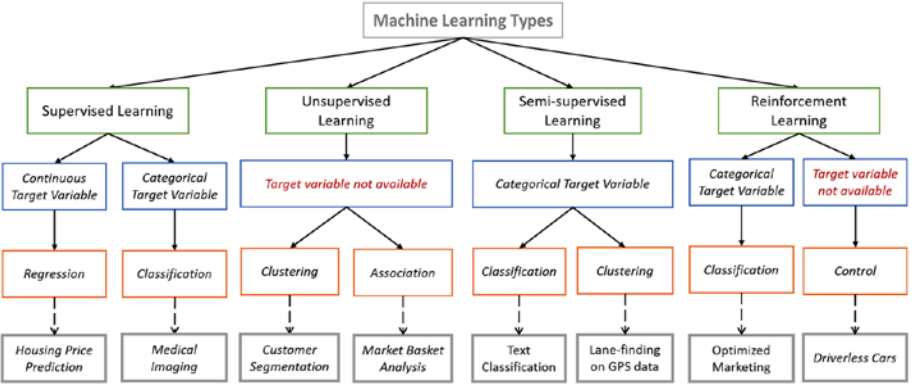
\includegraphics[width=\textwidth]{images/MachineLearningTypes_all}}
\caption{Machine Learning Types nach  \citep[S.~222]{ramasubramanian_machine_2017}}
\label{fig:MachineLearningTypes_all}
\centering
\end{figure}


\begin{table}[H]
\tiny
\begin{tabular}{|l|l|}
\hline
\textbf{Gruppe} & \textbf{Algorithmen}\\ 
\hhline{==}
Regression Analysis & Ordinary Least Square Regression (OLSR)\\
& Linear Regression\\
& Logistic Regression\\
& Stepwise Regression\\
& Polynomial Regression\\
& Locally Estimated Scatterplot Smoothing (LOESS)\\
\hline
Distance-based algorithms & k-nearest Neighbor (kNN)\\
& Learning Vector Quantization (LVQ)\\
& Self-Organizing Map (SOM)\\
\hline
Regularization algorithms & Ridge Regression\\
& Least Absolute Shrinkage and Selector Operator (LASSO)\\
& Elastic Net\\
& Least-Angle Regression (LARS)\\
\hline
Decision tree algorithms & Classification and Regression Tree (CART)\\
& Iterative Dichotomiser 3 (ID3)\\
& C4.5 and C5.0 (different versions of a powerful approach)\\
& Chi-squared Automatic Interaction Detection (CHAID)\\
& Random Forest\\
& Conditional Decision Tree\\
\hline
Bayesian algorithms & Naive Bayes\\
& Gaussian Naive Bayes\\
& Multinomial Naive Bayes\\
& Nayesian Belief Network (BNN)\\
& Bayesian Network (BN)\\
\hline
Clustering algorithms & k-Means\\
& k-Medians\\
& Partitioning Around Medoids (PAM)\\
& Hierarchical Clustering\\
\hline
Association rule mining & Apriori algorithm\\
& Eclat algorithm\\
& FP-growth algorithm\\
& Context Based Rule Mining\\
\hline
Artificial neural networks & Perception\\
& Back-Propagation\\
& Hopfield Network\\
& Radial Basis Function Network (RBFN)\\
\hline
Deep learning algorithms & Beep Boltzmann Machine (DBM)\\
& Deep Belief Networks (DBN)\\
& Convolutional Neural Network (CNN)\\
& Stacked Auto-Encoders\\
\hline
Dimensionality reduction algorithms & Principam Component Analysis (PCA)\\
& Principam Component Regression (PCR)\\
& Partial Least Squares Regression (PLSR)\\
& Multidimensional Scaling (MDS)\\
& Linear Discriminant Analysis (LDA)\\
& Mixture Discriminant Analysis (MDA)\\
& Quadratic Discriminant Analysis (QDA)\\
\hline
Ensemble learning & Boosting\\
& Bagging\\
& AdaBoost\\
& Stacked Generalization (blending)\\
& Gradient Boost Machines (GBM)\\
\hline
Text mining algorithms & Automatic summarization\\
& Named entity recognition (NER)\\
& Optical character recognition (OCR)\\
& Part-of-speech tagging\\
& Sentiment analysis\\
& Speec recognition\\
& Topic Modeling\\
   \hline
\end{tabular}
\caption{Sebjective Grouping nach \citep[S.~224-229]{ramasubramanian_machine_2017}}
\label{tab:SebjectiveGrouping}
\end{table}

Da der Artikel "How to choose algorithms for Microsoft Azure Machine Learning" von \citep{ericson_microsoft_2017} nach "Supervised", "Unsupervised" und "Reinforcement learning" zurückgreift, wird nachfolgend diese Gliederung genutzt und um "Semi-supervised Learning" und "Active Learning" erweitert. \newline
\todo{raus?:} Anzumerken ist, dass nur Algorithmen beschrieben werden, die zum Zeitpunkt der Arbeit in "Microsoft Azure Machine Learning Studio" verfügbar sind.

\subsection{Supervised Learning}
Die möglicherweise am einfachsten nachvollziehbare Gruppe des Machine Learning ist das Supervised Learning, da es "sehr ähnlich zu dem Prozess ist, in dem Menschen Dinge lernen"\citep[S.~13; eigene Übersetzung]{kim_matlab_2017}. Es existiert ein Datensatz, bei dem für jeden Input ein Output vorhanden ist. Ein Beispiel können Patientendaten sein, die als Output eine Variable besitzen, die angibt, ob ein Patient an Krebs erkrankt ist oder nicht.\citep[S.~222]{ramasubramanian_machine_2017} Diese "response variable" (Krebs oder nicht Krebs) wird als "label"\citep[S.~222]{ramasubramanian_machine_2017} bezeichnet. Die Aufgabe des Learning Prozesses ist es dann, einen Zusammenhang zwischen dem Input (Patientendaten) und dem Label (Krebs oder nicht Krebs) herzustellen. Dies geschieht mit sogenannten "training sets"\citep[S.~5]{paluszek_matlab_2017} Der zweite Schritt ist dann das Überprüfen des entstandenen Models. Dabei wird das Model auf ein zweites gelabeltes "test set"\citep[S.~5]{paluszek_matlab_2017} angewandt und das Ergebnis überprüft.\newline
Die Algorithmen des Supervised Learning lassen sich erneut aufteilen:

\subsubsection{Classification}
Betrachtet man die Labels und stellt fest, dass sie die Datensätze in Kategorien unterteilen (Krebs oder nicht Krebs) oder eine Wahrscheinlichkeit angeben (Person zu 89\% Max Mustermann bei einer Gesichtserkennung), handelt es sich um eine Klassifikation (engl. Classification).\citep[S.~67]{swamynathan_mastering_2017} \citep[S.~5]{kauchak_zoterovoll2.pdf_2016} nennt als Beispiele
\begin{itemize}
\item biometrische Erkennungen (Gesicht, Iris, Unterschrift etc.),
\item Buchstabenerkennung,
\item Spamfilter und
\item medizinische Diagnosen.
\end{itemize}
Weiterhin kann zwischen Klassifikationen mit nur zwei Labels ("two-class or binomial classification"\citep{ericson_how_2017}) (siehe Abbildung \ref{fig:classification}) oder mehr als zwei Labels ("multi-class classification"\citep{ericson_how_2017}) unterschieden werden.
\begin{figure}[H]
\frame{
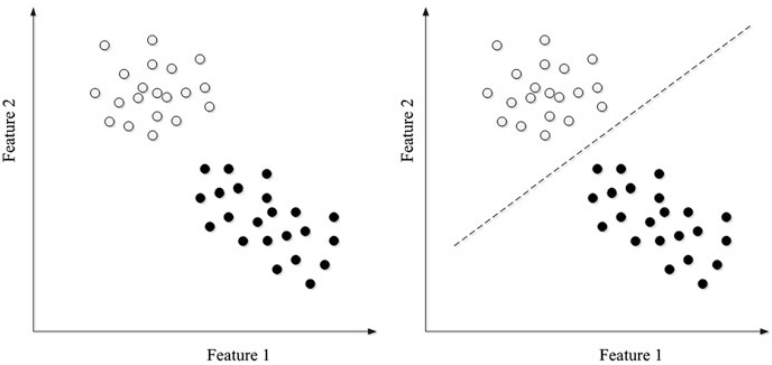
\includegraphics[width=\textwidth]{images/classification}}
\caption{Beispiel für eine Klassifikation aus \citep[S.~8]{suthaharan_machine_2016}}
\label{fig:classification}
\centering
\end{figure}
\subsubsection{Regression}
Wenn eine Unterteilung in Kategorien wie gerade genannt nicht möglich ist und die Output variable ein fortlaufender \todo{Wort} Wert ist, werden Regressionen benutzt. Dabei liegt der "Hauptfokus [...] darin, einen Zusammenhang zwischen einer abhängigen Variablen und einer oder mehreren unabhängigen [...] Variablen herzustellen"\citep[S.~60; eigene Übersetzung]{swamynathan_mastering_2017}. Neben dem bekanntesten Beispiel
\begin{itemize}
\item einen Kurs an der Börse vorherzusagen \multicitep{kauchak_zoterovoll2.pdf_2016, S.~5; kubat_introduction_2017, S.~207; ericson_how_2017}, gibt es Anwendungsfälle in
\item der Epidemiologie,
\item der Auto- und Flugzeugnavigation und
\item Analysen im zeitlichen Verlauf (Wetterveränderung im Verlauf der Zeit)\citep[S.~5]{kauchak_zoterovoll2.pdf_2016}.
\end{itemize}

\subsubsection{Anomaly detection}
Im bereits mehrfach zitierten Artikel "How to choose algorithms for Microsoft Azure Machine Learning" von \citep{ericson_how_2017} wird noch eine zusätzliche Kategorie genannte: Anomaly detection. Bei \citep[S.~68]{swamynathan_mastering_2017} ist die Anomaly detection dem Unsupervised Learning zugeordnet. Dies rührt daher, dass es darauf ankommt, ob eine Outputvariable ("Label") vorhanden ist, oder nicht. Tatsächlich ist es so, dass es sowohl Szenarien für Supervised und Unsupervised Anomaly detection gibt, als auch für das später noch beschriebene Semi-supervised Learning.\citep[S.~15:10]{chandola_anomaly_2009}
Unabhängig davon beschreibt Anomaly detection das Finden von Mustern in Daten, die vom erwarteten Verhalten abweichen. Diese Pattern werden meist als Anomalität (engl. anomaly) oder Ausreißer (engl. outliner) bezeichnet.\citep[S.~15:1]{chandola_anomaly_2009}
Die Anomaly detection kann für folgende Szenarien genutzt werden\citep[S.~15:2]{chandola_anomaly_2009}:
\begin{itemize}
\item Kreditkartenbetrugserkennung
\item Versicherungsbetrugserkennung
\item Gesundheitsprüfungen
\item Intrusion Detection
\item Militärische Überwachungen
\item Anwendungen in "der Welt des Internet der Dinge"[S.~68]\citep{swamynathan_mastering_2017}
\end{itemize}

\subsection{Unsupervised Learning}
Der "Glücksfall" \todo{kann man das so sagen?}, dass der vorhandene Datensatz Label besitzt, ist unter realen Umständen häufig nicht der Fall. Um aus diesen Daten trotzdem Schlüsse zu ziehen, werden Methoden des Unsupervised Learning herangezogen. Hier liegt der Fokus auf dem "Entdecken von aufschlussreichen Eigenschaften der verfügbaren Daten"\citep[S.277; eigene Übersetzung]{kubat_introduction_2017} und der "Untersuchung der Charakteristik der Daten"\citep[S.~13; eigene Übersetzung]{kim_matlab_2017}. Dies kann das Ziel haben komplexe und vielschichtige Daten zu vereinfachen und zu strukturieren\citep{ericson_how_2017} oder die Daten in Gruppen aufzuteilen\citep[S.~22]{lison_introduction_2012}. Um diese Gruppen ähnlicher Daten - sogenannte Cluster - geht es im nächsten Abschnitt.\newline
Supervised Learning findet man nach \citep[S.~223]{ramasubramanian_machine_2017}
\begin{itemize}
\item bei der Aufteilung von Kundendaten in Segmente,
\item in Analysen von sozialen Netzwerken,
\item in der Klimatologie,
\item bei der Bildkompression und
\item in der Bioinformatik.\citep[S.~6]{kauchak_zoterovoll2.pdf_2016}
\end{itemize}

\subsubsection{Clustering}
Beim angesprochenen Clustering handelt es sich um das "Identifizieren von distinkten Gruppen [...] basierend auf irgendeiner Art der Ähnlichkeit innerhalb des vorliegenden Datensatzes"\citep[S.~195; eigene Übersetzung]{swamynathan_mastering_2017}. Damit die Objekte der gebildeten Cluster "aussagekräftig und sinnvoll" sind, sollen "die Objekte innerhalb eines Clusters [...] homogen sein" und "zu Objekten anderer Cluster"\citep[S.~337; eigene Übersetzung]{ramasubramanian_machine_2017} heterogen (siehe Abbildung \ref{fig:clustering}). Es kann jedoch auch sein, dass Objekte zu mehreren Clustern gehören. Dies nennt sich "Soft Clustering" - im Gegensatz zum "Hard Clustering"\citep[S.~339]{ramasubramanian_machine_2017}. Die Metrik für die Ähnlichkeit ist nicht festgelegt. Möglich sind 
\begin{itemize}
\item die "Distanz [...] zwischen Beobachtungen", 
\item die "Entfernung vom Mittelwert jeder Beobachtung/des Clusters",
\item die "Signifikanz [einer] statistischen Verteilung" oder
\item die "Dichte im Datenraum"\citep[S.~338; eigene Übersetzung]{ramasubramanian_machine_2017}.
\end{itemize}
\begin{figure}[H]
\frame{
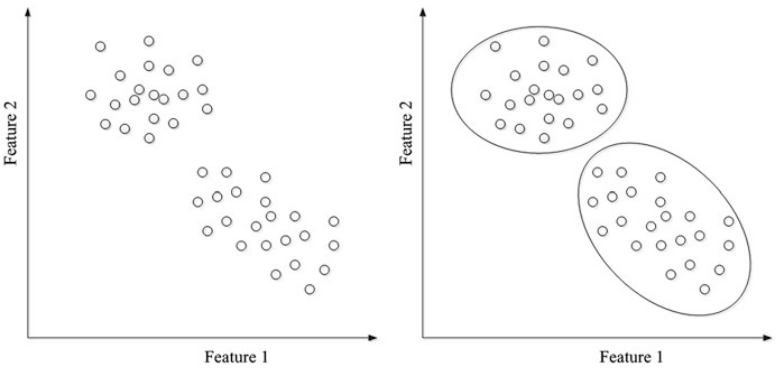
\includegraphics[width=\textwidth]{images/clustering}}
\caption{Beispiel für zwei Cluster \citep[S.~9]{suthaharan_machine_2016}}
\label{fig:clustering}
\centering
\end{figure}

\subsection{Semi-supervised Learning}
\todo{hier so oft "label...":}\newline
Bis jetzt wurden zwei Extremfälle beschrieben: entweder es gibt keine Labels oder alle Daten sind gelabelt. Es existieren jedoch auch Fälle dazwischen. Besitzen die meisten Daten ein Label, so ist es eventuell möglich, die Datensätze ohne Label für das Learning zu entfernen und ein Model aus dem Supervised Learning heranzuziehen. Tritt aber ein Problem auf, bei dem nur sehr wenige Daten gelabelt sind, empfiehlt sich ein Vorgehen aus dem Semi-supervised Learning. Methoden dieser Familie des Machine Learning beruhen auf der Annahme, dass "die Daten wichtige Informationen über die Gruppenzugehörigkeit beinhalten", "obwohl die Gruppenzugehörigkeit [...] unbekannt ist"\citep[S.~223; eigene Übersetzung]{ramasubramanian_machine_2017}. Als umfassendes Werk für Semi-supervised Learning ist an dieser Stelle \citep{chapelle_semi-supervised_2006} zu empfehlen. \newline
Zur Anwendung kommt Semi-supervised Learning seit den 1990er Jahre in "natural language problems" und "text classification"\citep[S.~4]{chapelle_semi-supervised_2006}.

\subsection{Active Learning}
Ein Sonderfall des Semi-Supervised Learning ist das Active Learning. Hier wird davon ausgegangen, dass nur wenige oder keine Labels vorhanden sind, diese jedoch durch einen "Menschen mit umfangreichem Wissen im Themengebiet"\citep[S.~i; eigene Übersetzung]{olsson_literature_2009} hinzugefügt werden können. Alle Daten mit einem Label zu versehen wäre jedoch zu "schwer, zeitaufwendig oder zu teuer"\citep[Abstract; eigene Übersetzung]{settles_active_2010}. Mit dem Ziel an den Menschen nur so wenig Anfragen (engl. Queries) wie nötig zu stellen\citep[Abstract]{olsson_literature_2009}, werden Algorithmen entworfen, die selbst wählen könne, welche Datensätze gelabet werden.\citep[Abstract]{settles_active_2010}\newline
Nach \citep[S.~4]{settles_active_2010} wird Active Learning beispielsweise in
\begin{itemize}
\item der Spracherkennung,
\item der Informationsextraktion oder in
\item der Klassifikation oder dem Filtern von Dokumenten oder Mediendateien eingesetzt
\end{itemize}

\subsection{Reinforcement Learning}
"Beim Reinforcement Learning interagiert der Lerner" - also ein Programm - "mit seiner Umwelt"\citep[S.~45; eigene Übersetzung]{settles_active_2010}. Er "experimentiert" dabei um eine Lösung auf das gestellte Problem zu finden und erhält je nach Ausgang seiner Aktion eine Belohnung oder eine Bestrafung.\citep[S.~331]{kubat_introduction_2017} Es wird also nicht direkt mit einem Output (Label) gearbeitet, sondern lediglich die Qualität des Outputs bewertet. Das Ziel ist, durch ein iteratives Vorgehen (siehe Abbildung \ref{fig:reinforcementLearning}), ein maximales Endergebnis (größer Reward) zu erreichen.\citep[S.~69]{swamynathan_mastering_2017}
\begin{figure}[H]
\frame{
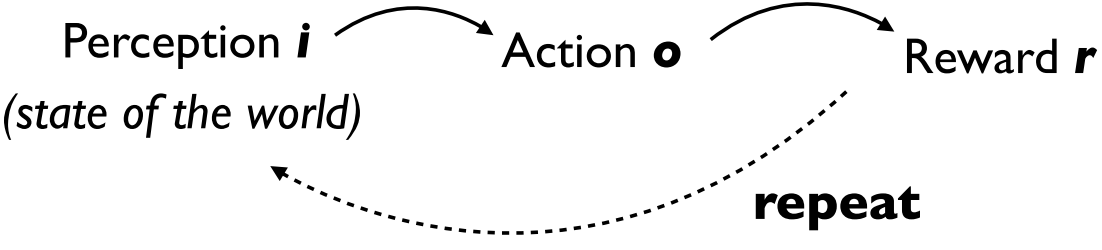
\includegraphics[width=\textwidth]{images/reinforcementLearning}}
\caption{Iterativer Reinforcement Learning Prozess aus \citep[S.~25]{lison_introduction_2012}}
\label{fig:reinforcementLearning}
\centering
\end{figure}
Reinforcement Learning kommt in Szenarien zum Einsatz, in denen noch keine Daten zum Lernen zur Verfügung stehen oder erst nach und nach aktualisiert werden.\citep[S.~223]{ramasubramanian_machine_2017}\newline
Ein prominentes Beispiel für ein System mit Reinforcement Learning ist Google DeepMinds AlphaGo. Es handelt sich dabei um einen Go (asiatisches Brettspiel) spielendes Computersystem, dass seine Spielstärke durch spielen gegen sich selbst erreichte.\citep{silver_mastering_2017}

\section{Krypotwährung(en)}
Bitcoin,ethereum, litecoin, dogecoin; auswahl hier nur 1/2


\section{SaaS}
\section{Microsoft Azure ML Studio}
\subsection{Allgemeine Beschreibung}
\subsection{Aufbau }
\subsubsection{Projects}
\subsubsection{Experiments}
\subsubsection{Web Services}
\subsubsection{Notebooks}
\subsubsection{Datasets}
\subsubsection{Trained Models}
\subsubsection{Settings}
\subsection{Elemente}
relevate auswählen
\subsubsection{Saved Datasets}
\subsubsection{Data Transformation Conversations}
\subsubsection{Data Transformation}
\subsubsection{Data Input and Output}
\subsubsection{Feature Selection}
\subsubsection{Machine Learning}
\subsubsection{OpenCV Library Models}
\subsubsection{Python Language Model}
\subsubsection{R Language Model}
\subsubsection{Statistical Functions}
\subsubsection{Text Analysis}
\subsubsection{Time Series Anomaly Detection}
\subsubsection{Web Service}
